\documentclass[12pt, a4paper]{article}
\usepackage{amsmath}
\usepackage{graphicx}
\usepackage[margin=1in]{geometry}
\usepackage[open]{bookmark} %pdf bookmarks
\usepackage{caption} % these 2 for subfigures
\usepackage{subcaption}
\usepackage{float} % for extra float options such as [H] after \begin{figure}
\linespread{1.3}
\setlength{\parindent}{0pt}
\setlength{\parskip}{\baselineskip}
\hypersetup{pdfstartview={XYZ null null 1.00}} % pdf zoom 100%

% \title{4A2 Computational Fluid Dynamics Interim Report}
% \author{}

\begin{document}

% \maketitle

\section{Results}
% \addcontentsline{toc}{section}{Section Name} to add unnumbered section to contents
\begin{figure}[H] %add [H] (float package) to 'override' float
	\centering
	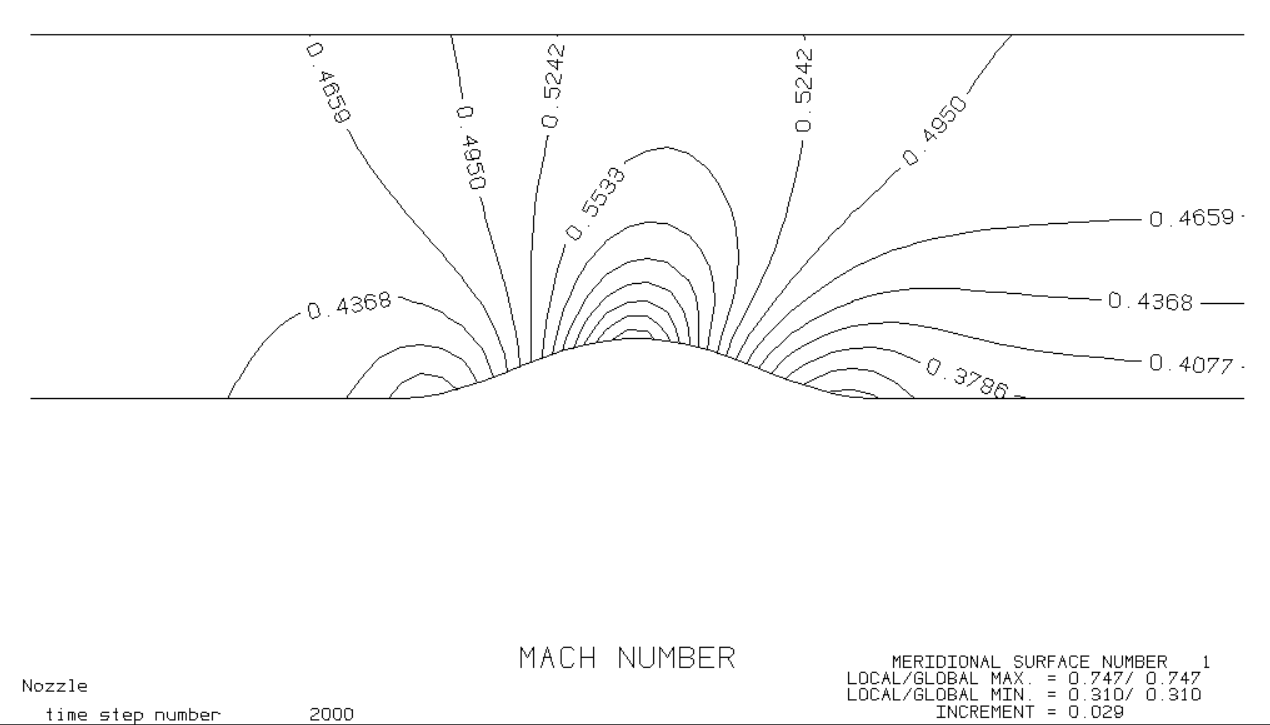
\includegraphics[width=\textwidth]{0mach}
	\caption{Mach number contour for test0}
	\label{fig:mach0}
\end{figure}
\begin{figure}[H]
	\centering
	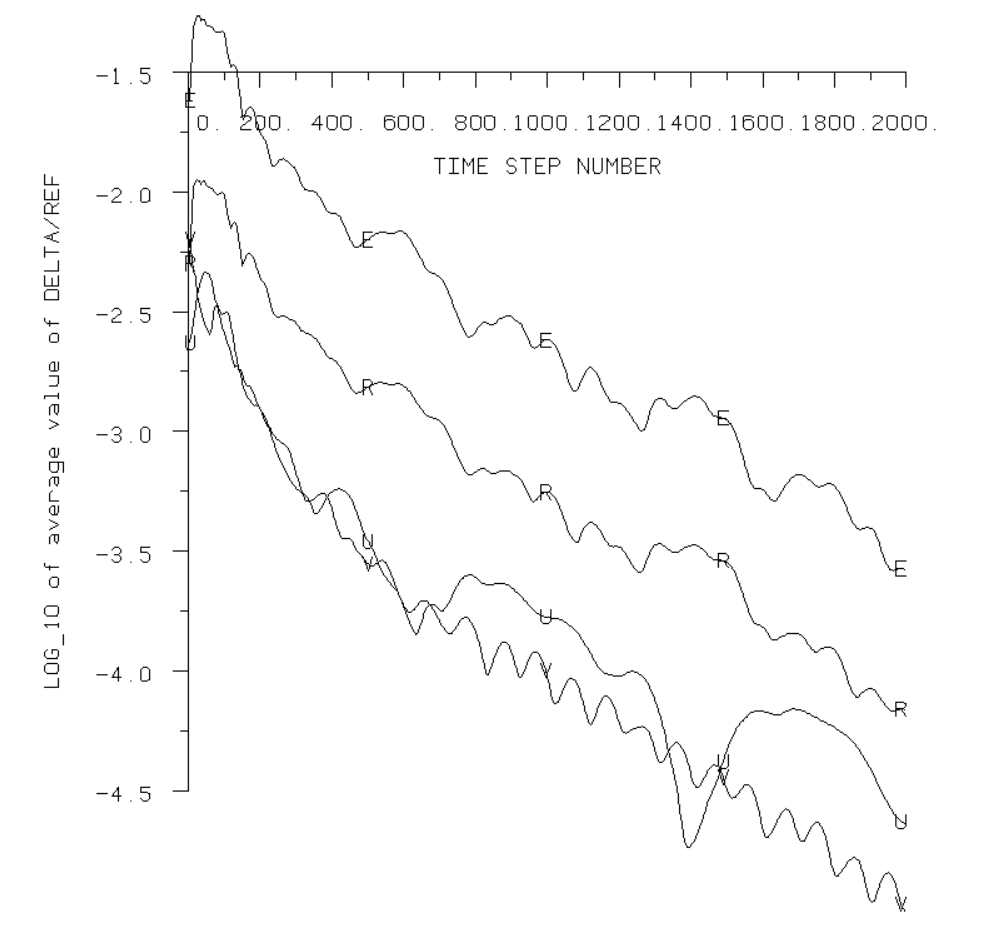
\includegraphics[width=0.75\textwidth]{0conv}
	\caption{Solution residual convergence for test0}
	\label{fig:conv0}
\end{figure}
\begin{figure}[H] %add [H] (float package) to 'override' float
	\centering
	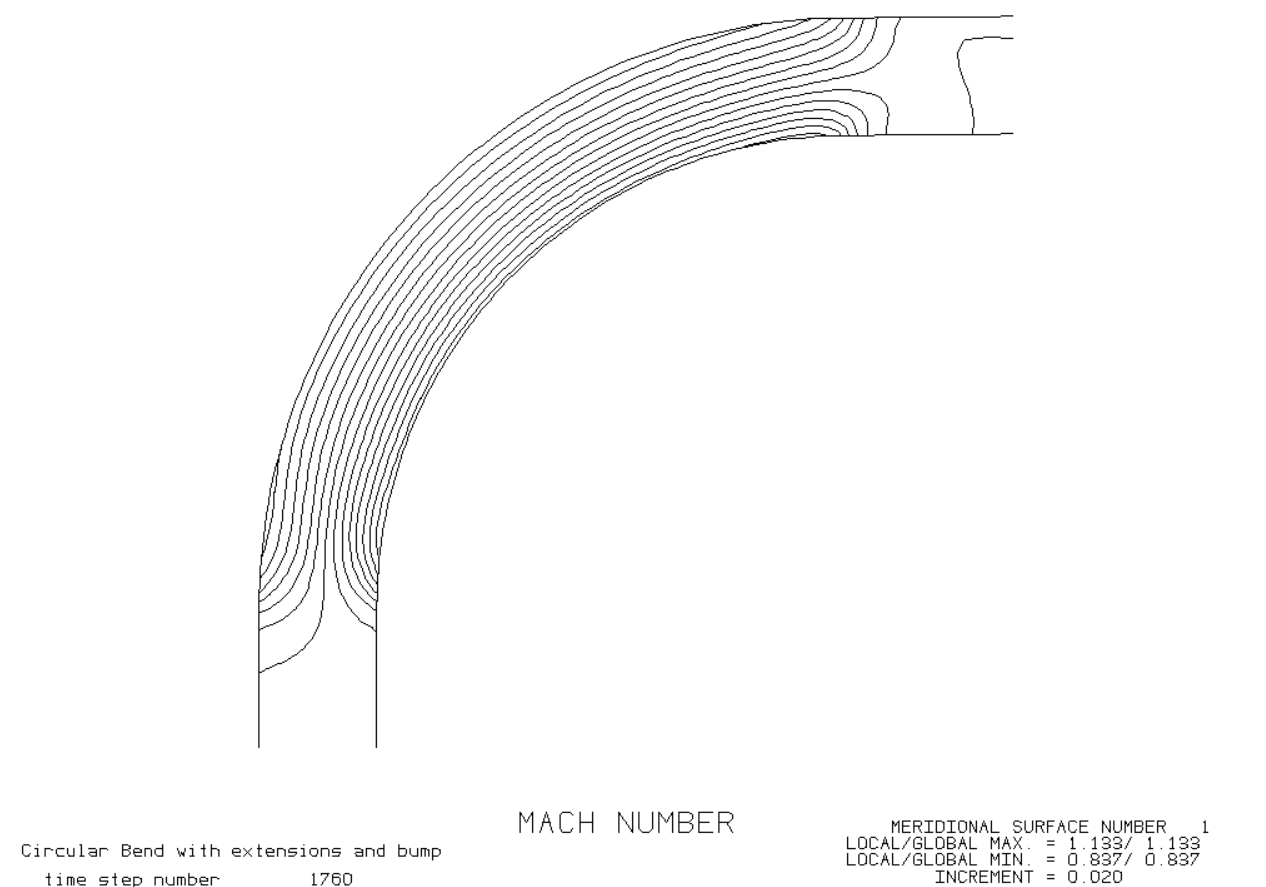
\includegraphics[width=\textwidth]{1mach}
	\caption{Mach number contour for test1}
	\label{fig:mach1}
\end{figure}
\begin{figure}[H]
	\centering
	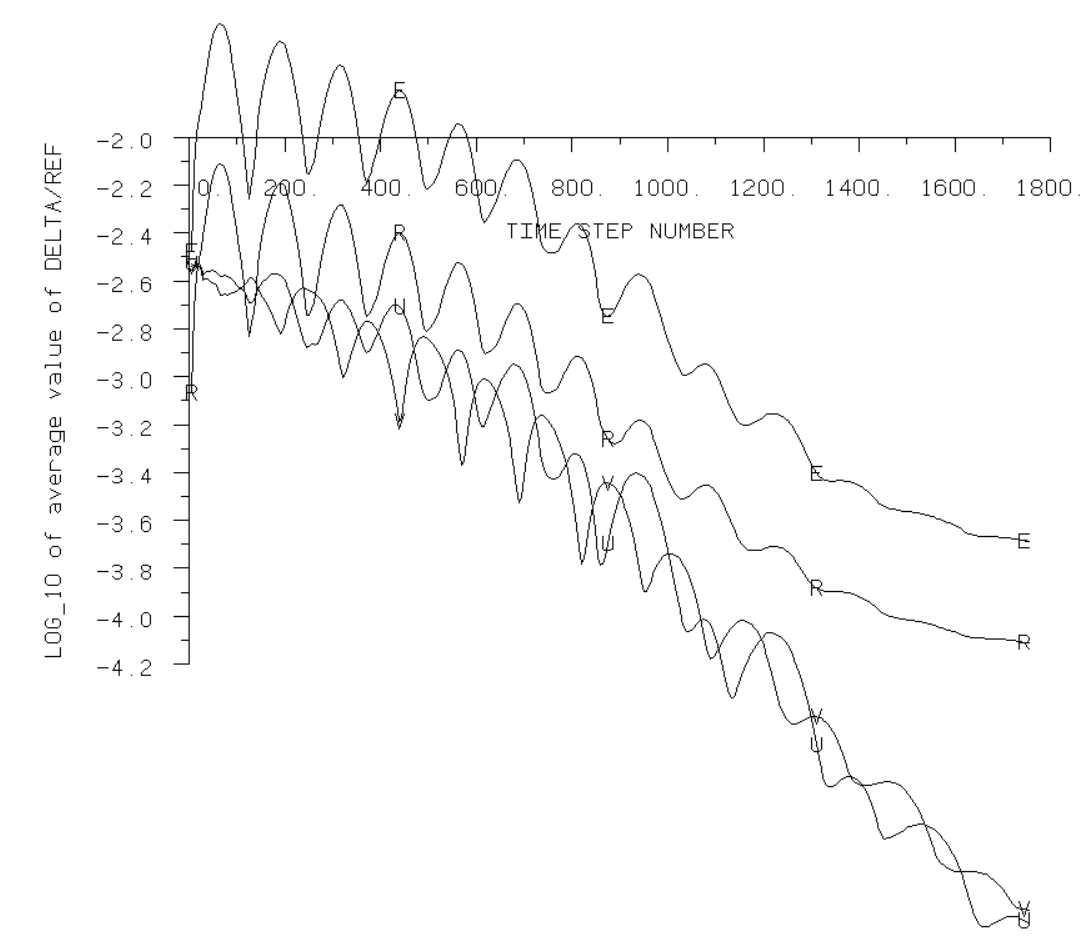
\includegraphics[width=0.75\textwidth]{1conv}
	\caption{Solution residual convergence for test1}
	\label{fig:conv1}
\end{figure}

For test0, the Mach contour results in Figure \ref{fig:mach0} match exactly with the 'Example Results' given on Moodle. A quick check for the outlet Mach number is by using the pressure ratios and assuming isentropic flow:
\begin{equation}\label{eq:mach}
	\dfrac{p}{p_0}=\left(1+\dfrac{\gamma-1}{2}M^2\right)^{-\dfrac{\gamma}{\gamma-1}}
\end{equation}

With the given downstream pressure ($pdown=85000\,Pa$) and inlet stagnation pressure ($pstagin=100000\,Pa$), $M_{outlet}=0.487$, which coincide with the results away from the bottom surface at the outlet. The maximum and minimum Mach number are the same with Example Results, follow the same shape and contour line values only vary by 0.0001. The solution using flow\_guess converged in 2000 time steps as opposed to the Example Result's 2040 time steps, suggesting the basic code is slightly more efficient in converging to a steady solution. In theory, this symmetrical geometry would lead to a symmetrical flow pattern. This is not the case because a smoothing factor was implemented in the numerical solution, which adds artificial diffusion. This makes the flow act as if there is viscosity.

For test1, the results are again identical to the Example Results. Similar accuracy assessments can be done, using the given downstream pressure ($pdown=50000\,Pa$) and inlet stagnation pressure ($pstagin=100000\,Pa$), Equation \ref{eq:mach} calculates $M_{outlet}=1.05$. This matches the result if the contour level is adjusted to see values. The solution converged in 1760 time steps compared to the Example Result's 1755. The convergence plot shows the average changes in each of the primary variables over the last 5 time steps, against time step number.Trends in the convergence graph match the Example Results. The slight asymmetry in the Mach plot is again due to artificial viscosity in the smoothing factor.

These 2 tests verify that the basic Euler solver code is correct. The code can now be developed further to improve efficiency, accuracy and speed. 

\section{1D Advection Python}
\begin{figure}[H]
	\begin{subfigure}[b]{0.48\textwidth}
		\centering
		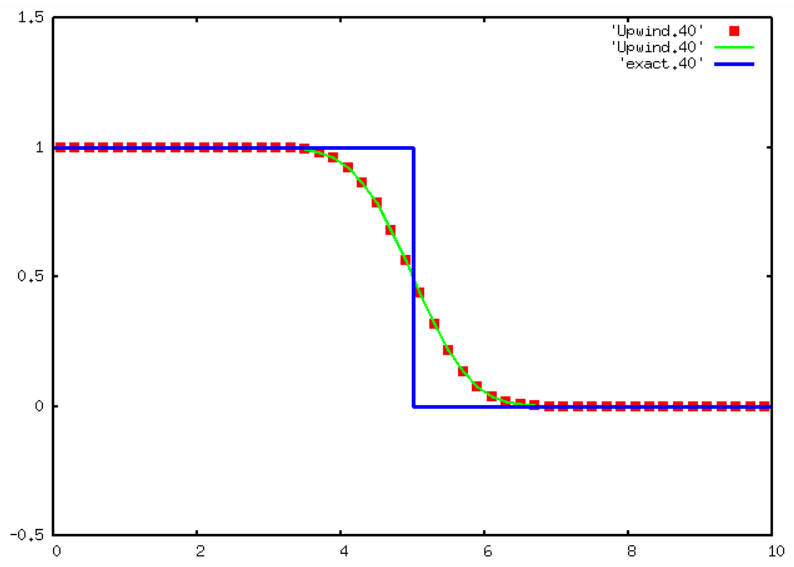
\includegraphics[width=\textwidth]{python/upwind}
		\caption{Upwind}
		\label{fig:upwind}
	\end{subfigure}
	\hfill
	\begin{subfigure}[b]{0.48\textwidth}
		\centering
		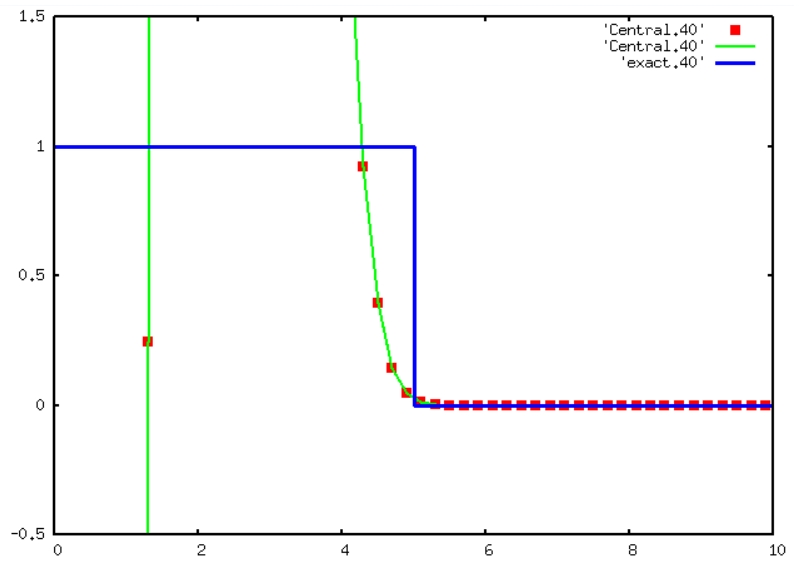
\includegraphics[width=\textwidth]{python/central}
		\caption{Central}
		\label{fig:central}
	\end{subfigure}
	\hfill
	\begin{subfigure}[b]{0.48\textwidth}
		\centering
		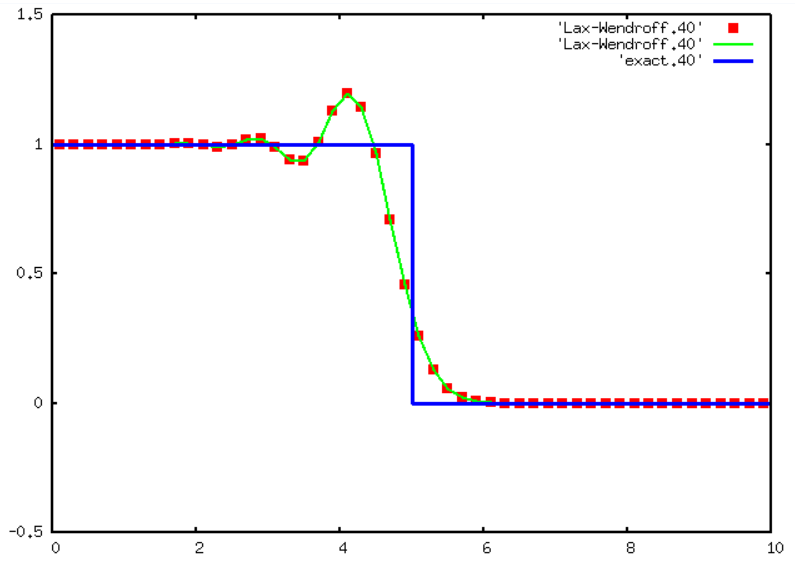
\includegraphics[width=\textwidth]{python/lax-wen}
		\caption{Lax-Wendroff}
		\label{fig:lax}
	\end{subfigure}
	\hfill
	\begin{subfigure}[b]{0.48\textwidth}
		\centering
		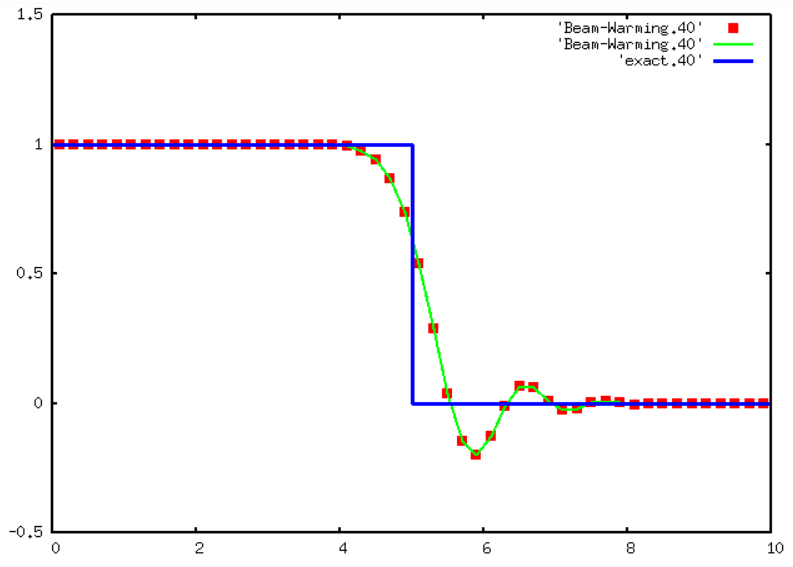
\includegraphics[width=\textwidth]{python/beam-warming}
		\caption{Beam-Warming}
		\label{fig:beam}
	\end{subfigure}
	\hfill
	\begin{subfigure}[b]{0.48\textwidth}
		\centering
		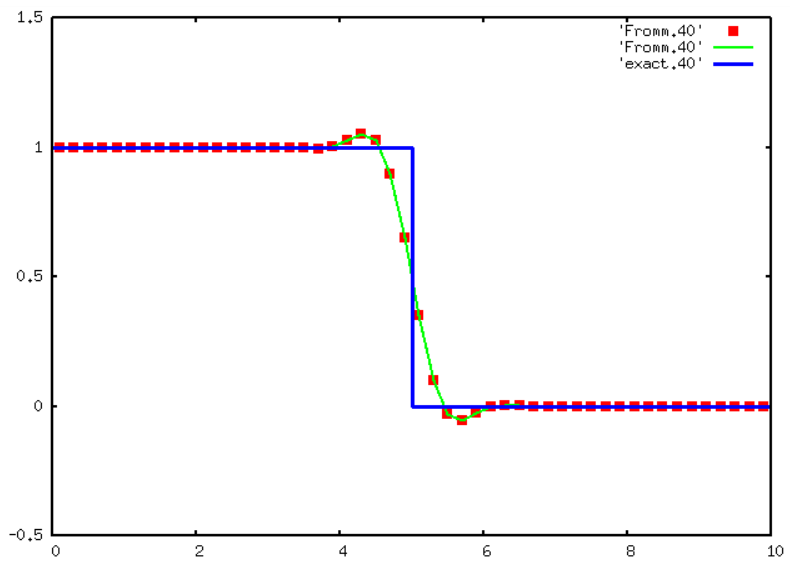
\includegraphics[width=\textwidth]{python/fromm}
		\caption{Fromm}
		\label{fig:fromm}
	\end{subfigure}
	\hfill
	\begin{subfigure}[b]{0.48\textwidth}
		\centering
		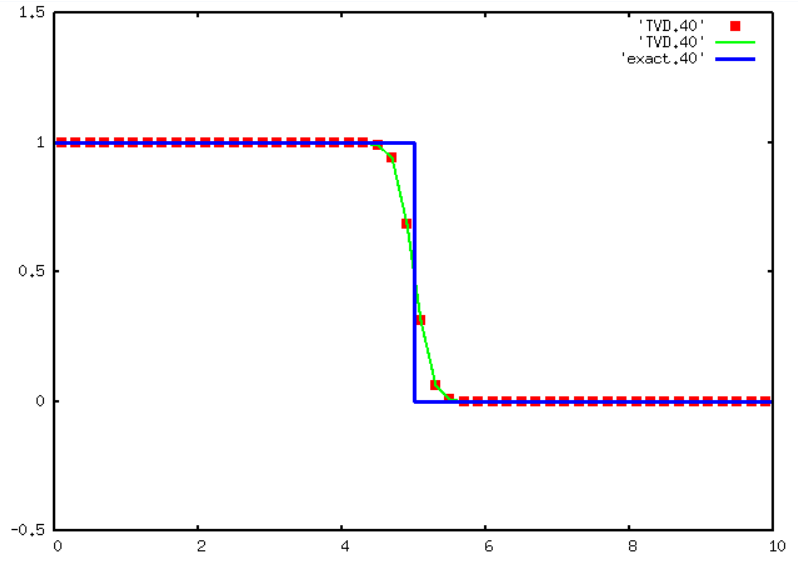
\includegraphics[width=\textwidth]{python/superbee}
		\caption{Superbee}
		\label{fig:superbee}
	\end{subfigure}
	\caption{1D Advection Python Solutions}
	\label{fig:advection}
\end{figure}

The upwind scheme in Figure \ref{fig:upwind} solves linear convection-diffusion equations. It is a first-order method which marches forward in time and upstream spacing. This solution is stable if the $CFL\le1$, as that implies the artificial diffusion has a non-negative viscosity in Equation \ref{eq:diffusion}, alternatively it means the n+1th point is in the characteristic's region of influence. However, the solution is very 'smeared' out compared to the exact solution. Truncation errors of even orders act like viscosity. The presence of this false diffusion in the numerical scheme leads to less accurate results, but does provide stability benefits by smoothing steep gradients in the exact solutions. The effective viscosity, or diffusion constant is obtained by using second-order Taylor Expansion and is given by:
\begin{equation}\label{eq:diffusion}
	D=\dfrac{a\Delta x}{2}(1-\dfrac{\Delta t}{\Delta x}a)
\end{equation}

The central space difference scheme is second-order in space, which makes it more accurate than the upwind method. However, as seen in Figure \ref{fig:central}, the solution diverges and is inherently unstable. This is because the solution depends on downstream values, which has incorrect physics as the flow also moves downstream. This leads to unstable solutions for all CFL numbers.

The Lax-Wendroff scheme uses second-order time difference Taylor Series, replacing time derivatives with spacial derivatives with the advection equation, and using central finite difference to replace the spacial derivatives. This eliminates the false diffusion which lead to a less smoothed and more closely matched solution. However, as this is now a third-order accurate scheme, there is now false convection (dispersion). The dispersive relation and stability constraints ($CFL<1$) mean the group velocity of all wave number travel too slowly, leading to the oscillations lagging behind the discontinuity as seen Figure \ref{fig:lax}.

The Beam-Warming scheme is very similar to Lax-Wendroff, in that it uses one-sided in place of the central difference formulae for the special derivatives. This leads to a modified dispersion relationship where group velocity for all wave numbers are greater than 'A' for $0<CFL<1$, so the oscillations move ahead of the discontinuity as seen in Figure \ref{fig:beam}. Again there is no false diffusion and the gradient matches more closely to the jump.

The Fromm scheme is a finite volume method based on piecewise linear reconstruction. It has a centred slope for the advection equation, obtaining second-order accuracy where the slope $\sigma_{i}^{n}$ approximates the derivative $q_x$ where q is a vector of conserved quantities. The reconstructed function is then advected in the positive direction, giving a nonsymmetric four-point formula. There is oscillations on either side of the discontinuity but are smaller than Lax-Wendroff and Beam-Warming, leading to a better approximated solution.

Lastly, the high order TVD method with a Superbee limiter is the best approximation to the exact solution out of all the methods shown here.  Superbee defines the limiter function as $\phi(\theta)=max(0,min(1,2\theta),min(2,\theta))$, where $\theta$ is a ratio measuring the smoothness of data locally. This gives a limiter function $\phi$ that has values near 1 for $\theta\approx1$ (high resolution), but that reduces the slope where the data is not smooth (low resolution). The lack of oscillations and smoothing means the error is very small and the gradient at the discontinuity is the steepest compared to the other methods.


\end{document}
